%------------------------------------------------------------------------------
% IPOL LaTeX style guide and Example
% by rafael grompone von gioi, nicolas limare, jose-luis lisani and others
%------------------------------------------------------------------------------

% IPOL class is based on the standard LaTeX article class is used
% essentially in the same way. The layout must not be changed. Special
% IPOL commands are used to set the title, authors and abstract.

\documentclass{ipol}

% Do not use math notations and greek letters in the title.
\ipolSetTitle{A MATLAB SMO Implementation to Train a SVM Classifier: Application to Multi-Style License Plate Numbers Recognition}

% Author names must be separated with commas (,), not "and" or "&".
\ipolSetAuthors{Pablo Negri\ipolAuthorMark{1}\ipolAuthorMark{2}}

% Affiliations must contain the department, institution and country.
% Use a professional email address (no gmail, yahoo, etc).
% Do not add postal address.
\ipolSetAffiliations{%
\ipolAuthorMark{1} CONICET, Godoy Cruz 2290, Buenos Aires, Argentina\\
\ipolAuthorMark{2} Instituto de Ciencias de la Computación (ICC), Departamento de Computación, Universidad de Buenos Aires, Buenos Aires, Argentina
                   (\texttt{pnegri@uba.dc.ar})}

%------------------------------------------------------------------------------

% The link hereafter points to IPOL documentation for convenience
% in this document but must be replaced in your manuscript.
% The preprint link will not be known before the first preprint page
% is created. For early preprint versions, just don't use this command
% and the link will be set to the IPOL journal DOI address.
\ipolPreprintLink{http://www.ipol.im/}

%------------------------------------------------------------------------------

% Add packages and definitions here.
% Keep the package list as small as possible and include the package
% sources (packagename.sty) with your article source.
% These packages are loaded by the IPOL class or considered standard,
% and need not be provided with their source if they are used:
%   color, hyperref, graphicx, rotating
%   amsmath, amssymb, amsthm
% For algorithms, please use the algorithm2e package instead of
% algorithmx for simplicity and a uniform style.

\usepackage[vlined,ruled]{algorithm2e}
% define input and output keywords
\SetKwInOut{Input}{input}
\SetKwInOut{Output}{output}
% define comment style
\SetKwComment{Comment}{}{}
\newcommand{\mycmtsty}[1]{\em \small #1}
\SetCommentSty{mycmtsty}

% Use \newtheorem{} for remarks and definitions.
\usepackage{amsthm}
\usepackage{amsmath}
\newtheorem{definition}{Definition}
\newtheorem*{remark}{Remark}

%------------------------------------------------------------------------------
\usepackage{slashbox}

\usepackage{fancyvrb}
\VerbatimFootnotes % allows verbatim text in footnotes

%%%%%%%%%%%%%%%%%%%%
\def\x{{\mathbf x}}
\def\v{{\mathbf v}}
\def\w{{\mathbf w}}
\def\E{{\mathbf E}}
\def\K{{\mathbf K}}
\def\C{{\mathbf C}}
%%%%%%%%%%%%%%%%%%%%
\DeclareMathOperator*{\argmax}{argmax}

\begin{document}

% IPOL encourages authors to do joint submissions to IPOL and
% SIIMS (SIAM Journal of Imaging Science). Upon acceptance, cross
% references are placed between both articles. The environment
% ipolSIIMS is used to set the standard header, before the
% abstract. Uncoment these lines if you prepare an IPOL+SIIMS article:

%\begin{ipolSIIMS}
%This IPOL article is related to a companion publication in the SIAM
%Journal on Imaging Sciences:\\
%Author Names, ``Article Title.''
%\textsl{SIAM Journal on Imaging Sciences}, vol.~X, no.~X,
%pp.~N--M, YYYY. \url{http://dx.doi.org/10.1137/XXXXXXXXX}
%\end{ipolSIIMS}

%------------------------------------------------------------------------------
% The abstract of an IPOL article must be informative and summarize all
% important parts of the article. 

\begin{ipolAbstract}
This paper implements the Support Vector Machine (SVM) training procedure proposed by John Platt denominated Sequential Minimimal Optimization (SMO).
The application of this system involves a multi-style license plate characters recognition identifying numbers from ``0'' to ``9''.
In order to be robust against license plates with different character/background colors, the characters (numbers) visual information is encoded using Histograms of Oriented Gradient (HOG).
A reliability measure to validate the system outputs is also proposed.
Several tests are performed to evaluate the sensibility of the algorithm to different parameters and kernel functions.
\end{ipolAbstract}

%------------------------------------------------------------------------------
% Use the source code info to briefly explain what can be found as
% software code in the IPOL article.
% Do not use the phrasing "...the IPOL web part of this article."

\begin{ipolCode}
The source code is written in MATLAB.
It implements the Platt's SMO algorithm to train and test a SVM classifier on a multi-style license plate character dataset.
Compilation and usage instruction are included in the \verb|README.txt| file of the archive.
The online demo allows to test the character (numbers) recognition system, from license plate images. 
\end{ipolCode}


%------------------------------------------------------------------------------
% Use the supplementary files info to add explanations about other
% files published with the article.

\begin{ipolSupp}
The supplementary files of the work includes a dataset of license plate numbers from four countries having different fonts, and character/background colors.
\end{ipolSupp}

%------------------------------------------------------------------------------
% All papers need key words. Key words are lowercase except for proper
% names and acronyms, and separated with commas. Only use plain text.

\ipolKeywords{Sequential Minimal Optimization, Support Vector Machine, Multi-Style License Plate Recognition, Histogram of Oriented Gradient}

%------------------------------------------------------------------------------
% Article content starts here.

\section{Introduction}

Sequential Minimal Optimization (SMO) \cite{Platt:1998} can be considered as the simplest algorithm to train a Support Vector Machine (SVM) classifier.
It uses the \textit{divide and conquer} approach to solve analytically a large quadratic programming (QP) optimization problem.
The reduction in complexity has several advantages: saving processing time and reducing memory consumption.
It is also a very interesting implementation that can be employed for pedagogical purposes, because the variables of the iterative algorithm can be easily accessed and interpreted in the learning process.

This paper uses SMO to implement a multi-class SVM classifier to address the problem of recognizing multi-style license plate numbers.
The One-Against-All approach is employed to classify the incoming characters from ``0'' to ``9''.
In order to be robust to changing colors and backgrounds, the features describing the characters' shape consist of Histograms of Oriented Gradients \cite{Dalal:2005}, as proposed by G\'{o}mez et al. \cite{Gomez:2011}.

%------------------------------------------------------------------------------
% Dataset and Feature Space

\section{Histogram of Oriented Gradient Feature Space}
The Histogram of Oriented Gradient (HOG) \cite{Dalal:2005} is a widely used image descriptor to successfully recognize different kinds of object classes, such as pedestrians, vehicles, etc.
It computes the gradient of the image $I(x,y)$, using, for example a 3x3 size Sobel filter, to get $(M(x,y),O(x,y))$, the matrices corresponding to the gradient magnitude and the gradient orientation, respectively.

The gradient directions are discretised into $D$ bins, and the histograms are determined by accumulating the gradient magnitude of each pixel of the region by their gradient directions. 
It is important to notice the gradient directions, not the gradient orientations, are used: Directions do not discriminate between dark-to-light and light-to-dark transitions.
Thus, the HOG feature set is independent of the character and background colors. 
We choose \textit{D} = 6.
Each HOG feature describing a region of the image is a histogram of $D$ bins.

Each histogram $j$ is defined as : $h_j (x_j,y_j,s_j,r_j)$, where $r_j$ is the type of rectangle, $s_j$ is the scale and $(x_j,y_j)$ is its position in the window.
The types of rectangles depend on the $(width,height)$ ratio which can be $(s,s)$, $(s,s/2)$, $(s/2,s)$. We have a total of four scales : $s:\{4,6,8\}$.

\begin{algorithm}[!htbp]
\small
\caption{HOG feature $j$}
\DontPrintSemicolon
\Input{$(M,O,x_j,y_j,s_j,r_j)$}
\Output{$h_j$}
$R \Leftarrow defineRectanglePositions(x_j,y_j,s_j,r_j)$ \\
Initialize $h_j$ as a zero vector of length $D$ \\
\ForAll{pixels positions $(x,y) \in R$} {
	$o = mod(round(D \cdot O(x,y)/ \pi),D) + 1$ \\
  $h_j(o) = h_j(o) + M(x,y)$ \\
}    
$T=\sum_{k=0}^{D-1}h_j(k)$ \\
\For{$k \leftarrow 0$ \KwTo $D-1$} {$h_j(k) = h_j(k) / T$} 
\label{alg:hog}
\end{algorithm}

Each histogram $h_j$ is computed using algorithm \ref{alg:hog}.
The function \textit{defineRectanglePositions()} transforms $r_j$ position and size from a normalized character pattern with a size of 16x12 pixels to their relative values in the input image shape.
Thus, it is not necessary to resize the image to compute each histogram.
Once all the pixels inside region $R$ have been evaluated and accumulated on $h_j$, the \textit{bin} values are normalized to sum 1.

Fig. \ref{fig:HoG} shows two samples from an Argentinean and an American license plate HOG features, with $D=6$, computed on regions with two different rectangles.
The green rectangle corresponds to a square feature and the red one is a vertical rectangle feature.
As can be seen, both HOG features are very similar for the two different license plate numbers.

\begin{figure}[!htbp]
\begin{center}
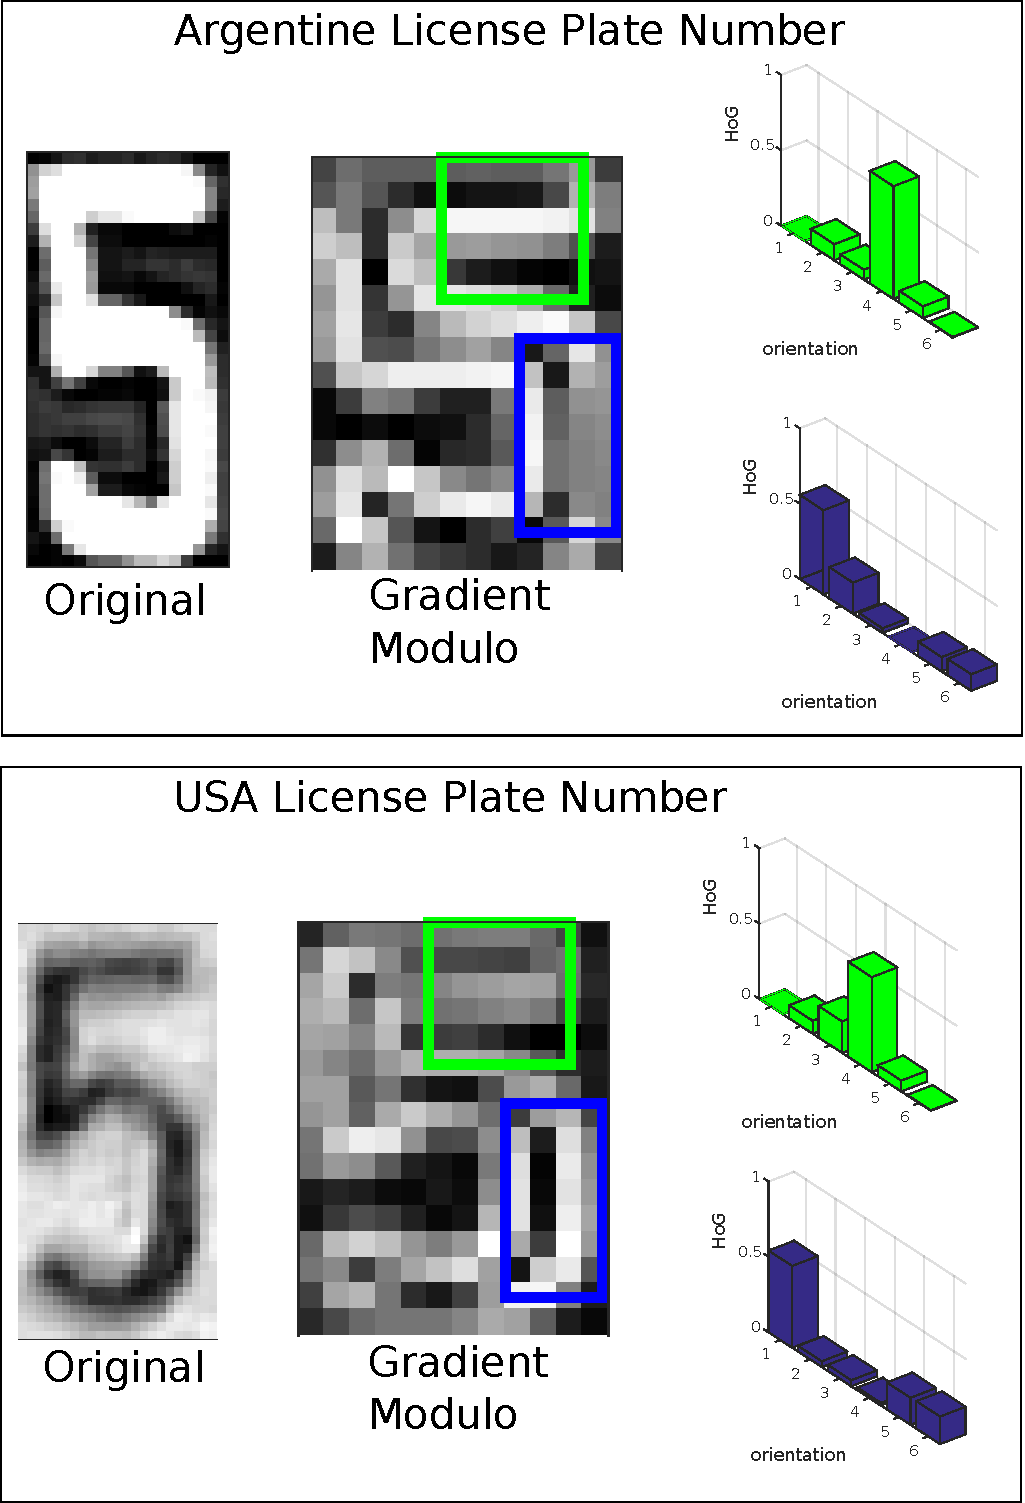
\includegraphics[width=.6\linewidth]{HoG.pdf}
\caption{The figure shows the same HOG features computed for two samples from different datasets.}
\label{fig:HoG}
\end{center}
\end{figure}

To accelerate the computation of the histograms, we use ``Integral Histogram'' \cite{Porikli:2005} which is an intermediate representation of the input image inspired by Viola \& Jones \textit{Integral Image} \cite{Viola:2004}. 
The Integral Histogram is a three dimensional table (the third dimension corresponds to orientations) that makes it possible to accumulate the gradient magnitude for each orientation in a rectangular region with only four references to it. 
Thus, each HOG feature can be built with $4 \times D$ access in the Integral Histogram.

Based on the 16x12 pixels pattern size, and computing overlapped rectangles $r_j$ with a displacement of one pixel, a set of 871 rectangles is obtained.
The descriptor of one character results in a vector $\x$ of $G=871$ concatenated histograms. 
This vector, of $G \times D$ values $\in \Re$, will be the input of the SVM multi-class classifiers.


%------------------------------------------------------------------------------
% SVM - SMO implementation

\section{SVM-SMO Implementation}

This section gives a very brief introduction to SVM classification and does not intend to be a guide of SVM learning or convex optimization.
Interested readers on those subjects can have a look at \cite{Burges1998,Cortes:1995,Scholkopf:2002}.
Here, the principal results for the non-linear case are presented and how the analytic solution is implemented.
The idea is to deduce the equations which will be employed on the Platt's pseudo-code for the sake of completeness of the Sequential Minimal Optimization methodology.
This description follows the presentation proposed in \cite{Platt:1998}, section 1.1.
Considering that Platt’s work gives a limited explanation of some equations, the procedure is completed based on \cite{Scholkopf:2002}, section 10.5. 


\subsection{SVM Introduction}

Vapnik \cite{Vapnik:1995} introduces Support Vector Machines as an optimization algorithm seeking to find the hyperplane with the maximum margin discriminating two classes on a dataset, as shown on Fig. \ref{fig:svm_margin}.

\begin{figure}[!htbp]
\begin{center}
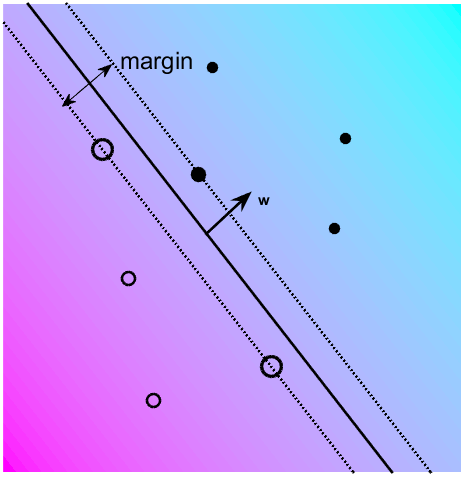
\includegraphics[width=.5\linewidth]{svm_margin.png}
\caption{The figure shows a toy sample of the SVM margin and a hyperplane definition in a two-class problem. The figure was produced using the demo code from \cite{Scholkopf:2002}.}
\label{fig:svm_margin}
\end{center}
\end{figure}

In its general form, the decision function that evaluates an input sample $\x_t$ is:
\begin{equation}\label{eq:svmoutput}
f(\x_t)= sign \left(\sum_{i=1}^N y_i \alpha_i K(\x_t,\x_i)-b\right)
\end{equation}

\noindent where the couples $\{\x_i,y_i\}_{i=1,...,N}$ corresponds to the training samples.
$\x_i \in \Re^d$ is the input vector from sample \textit{i} with size \textit{d}, and $y_i$ is the associated label that takes two possible values: -1 and 1. 
$K(\x_t,\x_i)$ is a kernel function estimating the similarity between sample $t$ and $i$ on the feature space.
Examples of kernel functions will be presented at section \ref{sec:evalparams}.
The constant $b$ is the threshold of the function.
The values of coefficients $\alpha$ correspond to the Lagrange multipliers of a quadratic programming (QP) problem. 
They are found by minimizing the following objective function:

\begin{equation}\label{eq:kernelObjetiveFunction}
\begin{aligned}
& \underset{\alpha \in \Re^N}{\text{minimize}}
& & \Psi(\alpha)=\frac{1}{2} \sum_{i=1}^N \sum_{j=1}^N y_i y_j K(\x_i,\x_j)\alpha_i \alpha_j - \sum_{i=1}^N \alpha_i \\
& \text{subject to}
& & 0 \leq \alpha_i \leq C, \forall i, \\
&\text{and}&&\sum_{i=1}^N y_i \alpha_i = 0.
\end{aligned}
\end{equation}

\noindent where the constant $C$ determines a compromise between margin maximization and training error minimization.
A large value for $C$ involves a high penalization on errors.

When the number of training samples is very small, the Support Vector optimization problem can be solved analytically.
In that case, the solution of eq. \ref{eq:kernelObjetiveFunction} involves the inversion of a Hessian matrix of size $N \times N$ \cite{Burges1998}.
For large datasets, the manipulation of this matrix becomes intractable in memory and time requirements.

The efforts were then conducted to divide the QP problem into a series of smaller QP sub-problems.
Vapnik \cite{Vapnik:1982} proposes a technique known as \textit{chunking} which relies on the fact that training samples with $\alpha_i=0$ are not involved with the solution of the QP problem.
The QP sub-problems use a subset of the non-zero $\alpha_i$ and the $M$ training samples that violates the most the  Karush-Kuhn-Tucker conditions (KKT):

\begin{equation} \label{eq:kktconditions}
\begin{aligned}
\alpha_i=0 \Rightarrow y_i f(\x_i) \geq 1 \\
0 < \alpha_i < C \Rightarrow y_i f(\x_i) = 1 \\
\alpha_i = C \Rightarrow y_i f(\x_i) \leq 1 \\
\end{aligned}
\end{equation}

With the obtained solution, the valued of the $\alpha_i$ are updated and a new subset is selected.
The algorithm finishes when the entire set of non-zero $\alpha_i$ is identified.

Osuna \cite{Osuna:1997} also reduces the QP problem into QP sub-problems with a fixed size Hessian matrix, by removing samples and adding others which violate KKT conditions.
Joachims \cite{Joachims:1998} employs an heuristic to choose the samples to be used on the QP sub-problem.


%%%%%%%%%%%%%%%%%%%%%%%%%%%%%%%%%%%%%%%%%%%%%%%%%%%%%%%%%%%%%%%%%%%%%%%%%%%%%%%%%%%%%%%%%%%%%%%%%%%%%%%%%
\subsection{Sequential Minimal Optimization: Two Variable Analytic Solution}\label{sec:twovars}

SMO is a simple algorithm that push the \textit{chunking} method to the smallest possible expression by using only two-Lagrange-multiplier at each iteration.
It finds the optimal value for these multipliers, and updates the SVM framework, until the entire QP problem is solved.
The advantage of SMO is that for two Lagrange multipliers, the optimization sub-problem can be solved analytically.
This methodology is detailed below in this section.

The algorithm chooses two training samples ($\x_1$,$y_1$) and ($\x_2$,$y_2$).
Their associated Lagrange multipliers are $\alpha_1$ and $\alpha_2$.
For the sake of simplicity, the kernel function computation is expressed as $K(\x_1,\x_1)=K_{11}$, $K(\x_1,\x_2)=K(\x_2,\x_1)=K_{12}$, and $K(\x_2,\x_2)=K_{22}$.
For two variables $\alpha_1$ and $\alpha_2$, the optimization of objective function $\Psi(\alpha)$ from equation \ref{eq:kernelObjetiveFunction} becomes \cite{Scholkopf:2002}:

\begin{equation}\label{eq:twoVarOptimization}
\begin{aligned}
& \underset{\alpha_1,\alpha_2}{\text{minimize}}
& & \Psi(\alpha) = \frac{1}{2} (\alpha_1^2 K_{11} + 2 s \alpha_1 \alpha_2 K_{12} + \alpha_2^2 K_{22}) - \alpha_1 - \alpha_2 \\
& \text{subject to}
& & 0 \leq \alpha_1 \leq C, \\
&&& 0 \leq \alpha_2 \leq C, \\
&&& s \alpha_2 + \alpha_1 = \gamma 
\end{aligned}
\end{equation}

\noindent where $s=y_1 \cdot y_2$, $\gamma \in \Re$.

To solve the QP problem of eq. \ref{eq:twoVarOptimization}, the objective function $\Psi(\alpha)$ and the constraints are simplified with the substitution: $\alpha_1 = \gamma - s\alpha_2$.
Eq. \ref{eq:twoVarOptimization} is then rewritten as:

\begin{equation}\label{eq:oneVarOptimization}
\begin{aligned}
& \underset{\alpha_2}{\text{minimize}}
& &  \Psi(\alpha) = \frac{1}{2} \alpha_2^2 ( K_{11} + K_{22} - 2 K_{12}) + \alpha_2 ( s \gamma K_{12} - s \gamma K_{11} + s - 1) + \frac{\gamma^2 K_{11}}{2} - \gamma \\
& \text{subject to}
& & 0 \leq \alpha_2 \leq C, \\
&&&\gamma - C \leq \alpha_2 \leq \gamma, \ (\textrm{if }s=1) \\
&&& - \gamma  \leq \alpha_2 \leq - \gamma + C, \ (\textrm{if }s=-1).
\end{aligned}
\end{equation}

\noindent where constraints on $\alpha_2$ are related to constraints on $\alpha_1$, from equation \ref{eq:twoVarOptimization}.
The optimization problem will now be solved for $\alpha_2$.

The quadratic objective function $\Psi(\alpha_2)$ on eq. \ref{eq:oneVarOptimization} has the form:
\begin{equation}
\Psi(\alpha_2) = \frac{\chi}{2}\alpha_2^2 - \zeta \alpha_2 + \kappa \label{eq:zeroEq}
\end{equation}

\noindent with
\begin{eqnarray}
\zeta & = & s \gamma K_{11} - s \gamma K_{12} - s + 1 \\
\chi & = & K_{11} + K_{22} - 2 K_{12} \\
\kappa & = & \frac{\gamma^2 K_{11}}{2} - \gamma
\end{eqnarray}

The  minimal $\alpha_2$ of \ref{eq:zeroEq} is the root of:
\begin{equation}\label{eq:derivada}
\frac{\partial \Psi(\alpha_2)}{\partial \alpha_2} = \chi \alpha_2 - \zeta = 0
\end{equation}

\noindent which is is placed at $\alpha_2=\chi^{-1}\zeta$.
This value, however, must to be clipped into the constrains in eq. \ref{eq:oneVarOptimization}.
Both constrains can be combined on the interval $L \leq \alpha_2 \leq H$ using: 

\begin{equation}
L = \left\{ \begin{array}{l r}
max(0,s(\gamma - C)) & \textrm{if }s = 1 \\
max(0,s\gamma) & \textrm{otherwise}
\end{array}
\right.
\end{equation}

\begin{equation}
H = \left\{ \begin{array}{l r}
min(C,s\gamma) & \textrm{if }s = 1 \\
min(C,s(\gamma-C)) & \textrm{otherwise}
\end{array}
\right.
\end{equation}

The value of $\alpha_2$, solution of eq. \ref{eq:derivada}, is computed considering two cases:

\noindent \textit{Case 1: }$\chi = 0$\\

\begin{equation}
\alpha_2 = \left\{ \begin{array}{l r}
H & \textrm{if }\zeta > 0 \\
L & \textrm{otherwise}
\end{array}
\right.
\end{equation}

\noindent \textit{Case 2: }$\chi > 0$\\

\begin{equation}
\alpha_2 = min(max(L,\chi^{-1} \zeta),H)
\end{equation}

\noindent Case $\chi < 0$ occurs when two training samples have the same feature vector.
To avoid this situation, a preliminary step eliminating duplicated inputs is then mandatory.

It can be proved that the new value of $\alpha_2$ gets the minimal values along the direction of the constrains by using the following equation (see \cite{Scholkopf:2002}, Proposition 10.4):

\begin{equation}\label{eq:itrativealpha2}
\alpha_2^{new}=\alpha_2^{old} + \frac{y_2 (E_1-E_2)}{\chi}
\end{equation}

\noindent where $E_i=f(\x_i)-y_i$ is the error evaluating the $ith$ sample with eq. \ref{eq:svmoutput}.
This value of $\alpha_2^{new}$ has to be \textit{clipped} to assure that the value will lie between the constraints:

\begin{equation}\label{eq:clippedvalues}
\alpha_2^{new,clipped} = \left\{ \begin{array}{l c r}
H & if & \alpha_2^{new} \geq H \\
L & if & \alpha_2^{new} \leq L \\
\alpha_2^{new} & otherwise & \\
\end{array}
\right.
\end{equation}

Finally, the value of $\alpha_1^{new}$ is then obtained from $\alpha_2^{new,clipped}$ as follows:

\begin{equation}
\alpha_1^{new} = \alpha_1^{old} + s(\alpha_2^{old} - \alpha_2^{new,clipped})
\end{equation}
%%%%%%%%%%%%%%%%%%%%%%%%%%%%%%%%%%%%%%%%%%%%%%%%%%%%%%%%%%%%%%%%%%%%%%%%%%%%%%%%%%%%%%%%%%
%%%%%%%%%%%%%%%%%%%%%%%%%%%%%%%%%%%%%%%%%%%%%%%%%%%%%%%%%%%%%%%%%%%%%%%%%%%%%%%%%%%%%%%%%%
\subsection{Implementation of the Sequential Minimal Optimization Algorithm}\label{sec:smo}

Platt's paper \cite{Platt:1998} proposes the pseudo-code of some routines to solve the SMO algorithm.
Here, the pseudo-code is highly inspired from \cite{Platt:1998}, and also follows the MATLAB implementation code that supports this article.

Algorithm \ref{alg:mainroutine} shows the \textit{Main Routine} that initializes the SVM training algorithm for a two classification problem.
The inputs of the procedure are the following:
\begin{itemize}
\item Training Dataset: composed of $N$ pairs $(\x_i,y_i)$, where $N$ is the length of the dataset, $\x_i$ is the feature vector of sample $i$, and $y_i$ is the target of sample $i$ corresponding to the following labels: ${1,-1}$, indicating to which it belongs.
\item Kernel Matrix Function $\mathbf{K}$: this is a two dimensional $N$x$N$ matrix. 
Each element $(i,j)$ from the matrix consists of the output of the non-linear kernel function $K(\x_i,\x_j)$.
\item $C$ parameter: the SVM training is very sensitive to this parameter.
Generally, its value is computed by a k-fold cross validation approach, choosing the value which maximizes the results in a validation set.
\item Initial $b$ parameter: bias threshold parameter of the SVM hyperplane. It is initialized to 0.
\item $\E$ error vector: this vector stores the errors of the training samples: $E_i = f(\x_i) - y_i$, where $f_i$ is computed using equation \ref{eq:svmoutput}.
The initial values of the elements are: $E_i = - y_i, \forall i$.
This vector will be updated every time that a Lagrange multiplier changes its value, because $f_i$ also changes.
\item Initial $\mathbf{\alpha}$ vector: the values of the Lagrange multipliers $(\alpha_i)$, with $i=1,...N$, are initialized to zero. 
\end{itemize}

\begin{algorithm}[!htbp]
\small
\caption{Main Routine}
\DontPrintSemicolon
examineAll = 1\\
numChanged = 0\\
\While{examineAll OR numChanged $>$ 0}{
numChanged = 0\\
	\If {examineAll} {
		\ForAll{element $i$ of the training set} {
			numChanged = numChanged + examineExample($i$)
			}
			examineAll = 0 \\
		}
		\Else {\ForAll{element $i$ of the training set where $0 <\alpha_i<C$} {
			numChanged = numChanged + examineExample($i$)
			}
			examineAll = 1 \\
		}
}
\label{alg:mainroutine}
\end{algorithm}

Algo \ref{alg:mainroutine} is the main script that evaluates all the samples and their associated Lagrange multipliers $\alpha_i$.
This procedure calls the \textit{examineExample()} routine which optimizes and updates the Lagrange multipliers.
\textit{numChanged} accumulates the number of multipliers updated at each iteration by the function \textit{examineExample()}.
The routine converges when the values of the multipliers have not changed in a whole iteration.
The output of the procedure is the list of Lagrange multipliers $\alpha_i$ and bias $b$.
In combination with training samples $\x_i$, and targets $y_i$, any incoming test sample can be evaluated using equation \ref{eq:svmoutput}.



The \textit{examineExample} routine (algorithm \ref{alg:examineExample}) iteratively chooses all the samples from the training set and searches another sample to update its Lagrange multipliers.
At the end of the cycle, if the values of the multipliers have converged, the algorithm stops.

\begin{algorithm}[!htbp]
\small
\caption{examineExample()}
\DontPrintSemicolon
\Input{$i$ index sample}
\Output{flagChanges}
$r_i = E_i \cdot y_i$\\
\If{($r_i$ $<$ -tol AND $\alpha_i$ $<$ $C$) AND ($r_i$ $>$ tol AND $\alpha_i$ $>$ $0$)} {
	\If{exists $j \neq i$  with $0 < \alpha_j < C$  } {
		$j$ = secondChoiceHeuristic($i$) \\
		\If {takeStep($j$,$i$)} {
			return 1\\
		}
		\ForAll{remaining examples $j \neq i$ with $0 < \alpha_j < C$} {
			$j$ = randomly picked example \\
			\If {takeStep($j$,$i$)} {
				return 1\\
				}
		}
	}
	\ForAll{possible indexes $j$ on train dataset} {
		\If {takeStep($j$,$i$)} {
			return 1\\
		}
	}
}
return 0\\
\label{alg:examineExample}
\end{algorithm}

Each time that \textit{examineExample()} picks one training sample $i$, it is necessary to choose another sample $j$ to solve the optimization problem for two multipliers.
Platt proposes a heuristic to identify sample $j$ so as to maximize the numerator of eq. \ref{eq:itrativealpha2}.
This methodology, referred to as \textit{Second Heuristic}  seeks to find the pair of samples where the difference in the classification error is significant, and there is still place for improvement conditioned to the Lagrange multipliers.

\begin{algorithm}[!htbp]
\small
\caption{secondChoiceHeuristic()}
\DontPrintSemicolon
\Input{$E$,$i$}
\Output{$j$}
sE,sidx = sort values of error vector E \\
\If {$E_i$ $>$ $0$} {
    \Comment{choose the sample with lowest error to maximize the step size $|E_i - E_j|$}
    \If {sidx[1] equals $i$} {$j$ = sidx[2]}
		\Else {$j$ = sidx[1]}
	}	
 \Else {   
   \Comment{choose the sample with highest error to maximize the step size $|E_i - E_j|$}
    \If {sidx[last] equals $i$} {$j$ = sidx[last-1]}
    \Else {$j$ = sidx[last]}
   }
	return $j$\\
\label{alg:secondChoiceHeuristic}
\end{algorithm}

Algorithm \ref{alg:takeStep} is function \textit{takeStep}, which updates the values of the Lagrange multipliers with indexes $i$ and $j$.
If the change between new and old values is considerable, bias threshold \textit{b} and error list \textit{E} are updated, using alg. \ref{alg:updateThreshold} and alg. \ref{alg:updateErrorList} respectively.
If the change is not noticeable, the function outputs a zero value (false) indicating this situation.
Section 2.3 of Platt's original work \cite{Platt:1998} details the methodology which update thresholds \textit{b}.

\begin{algorithm}[!htbp]
\small
\caption{takeStep()}
\DontPrintSemicolon
\Input{$j$,$i$}
\Output{$flagChanged$}
$s = y_i y_j$\\
\If{$y_j$ equals $y_i$ (s=1)} {
	L=max(0,$\alpha_i+\alpha_j-C$)\\
	H=min($C$,$\alpha_i+\alpha_j$)\\
	}
\Else {
	L=max(0,$\alpha_i-\alpha_j$)\\
	H=min($C$,$C+\alpha_i-\alpha_j$)\\
	}	
\If{the boundaries overlap (L=H)}
	{return 0}
$\chi = \K(j,j) + \K(i,i) - 2\K(j,i)$ \\

\If{$\chi > 0$}{
	$a_2 = \alpha_i + y_i \cdot \frac{(E_j-E_i)}{\chi}$ \\
	\If{$a_2$ $<$ L} {$a_2$ = L} 
	\ElseIf{$a_2$ $>$ H} {$a_2$ = H}	
}
\Else {
	\If{$(y_i \cdot (E_j-E_i)) < 0$} {$a_2$ = H}
	\ElseIf{$(y_i \cdot (E_j-E_i)) > 0$}{$a_2$ = L}
	\Else{$a_2$ = $\alpha_i$}
}
\If{$|a_2-\alpha_i|$ $<$ $eps \cdot (a_2+\alpha_i+eps)$}{return 0}
$a_1 = \alpha_1 + s \cdot (\alpha_i-a_2)$\\
updateThreshold($j$,$i$,$a_1$,$a_2$)\\
$\alpha_j$ = $a_1$\\
$\alpha_i$ = $a_2$\\
updateErrorList()\\
return 1\\
\label{alg:takeStep}
\end{algorithm}

\begin{algorithm}[!htbp]
\small
\caption{updateThreshold()}
\DontPrintSemicolon
\Input{$j$,$i$,$a_1$,$a_2$}
\Output{$b$}
$b_1 = E_j + y_j \cdot (a_1 - \alpha_j) \cdot \K(j,j) + y_i \cdot (a_2 - \alpha_i) \cdot \K(j,i) + b$\\
$b_2 = E_i + y_j \cdot (a_1 - \alpha_j) \cdot \K(j,i) + y_i \cdot (a_2 - \alpha_i) \cdot \K(i,i) + b$\\
$b = 0.5 (b_1+b_2)$ \\
\label{alg:updateThreshold}
\end{algorithm}


\begin{algorithm}[!htbp]
\small
\caption{updateErrorList()}
\DontPrintSemicolon
\Input{}
\Output{$E$}
\ForAll{element $i$ of the training set} {
	$u_i = \sum_{j=1}^N y_j \alpha_j \K(i,j) - b$ \\
	$E_i = u_i - y_i$ \\
}
\label{alg:updateErrorList}
\end{algorithm}

The output of the SMO learning algorithm are the values of $\alpha_i$, and bias $b$.
In order to test a new input sample using eq. \ref{eq:svmoutput}, these values are needed: feature vectors $\x_i$, and labels $y_i$ of the training samples.

The next section implements this algorithm to train a pool of classifiers which will recognize license plate numbers.

%--------------------------------------------------------------------------------------------
\section{Multi-class SVM Recognition Framework}

The License Plate Number recognition is considered as an $M=10$ multi-class problem.
This problem is solved using the One-Against-All approach \cite{Rifkin:2004,Liu:2005}.
%%%%%%%%%%%%%%%%%%%%%%%%%%%%%%%%%%%%%%%%%%%%%%%%%%%%%%%%%%%%%%%%%%%%%%%%%%%%%%%%%%%%%%
\subsection{SVM Multiclass Recognition Strategies}

SVM basically consists on a binary classifiers, generating a hyperplane which separates to classes from a training dataset.
Two of the most used strategies adapting SVM to multiclass tasks are: One-Against-One, and One-Against-All \cite{Milgram:2006,Gidudu:2007}.

Let be the training dataset composed of $N$ samples: $\{x_1,y_1\}, ...,\{x_N,y_N\}$.
Each $x_i \in \Re^d$ is the input vector of concatenated HOG features, and $y_i \in \{1,...,M\}$ is the corresponding label associated with one of the $M$ classes.
The One-Against-All approach trains separately $M$ binary SVM classifers, one class vs all the other classes: the machine corresponding to class $i$ is trained setting label $y=1$ to samples of the $i-th$ class, while the other samples get label $y=-1$.

Equation \ref{eq:svmoutput} then becomes:

\begin{equation}\label{eq:multisvmoutput}
f_i(\x_t)=\sum_{j=1}^N \mathbf{1}_{y_j=i} \alpha_{i,j} K(\x_t,\x_j)-b_i
\end{equation}

\noindent where notation $\mathbf{1}_{y_j=i}$ is the label function of $y_j$, which takes value $1$ when the sample has the same label as the training class, $y_j=i$, and $-1$; otherwise, variables $\{\alpha_{i,j},b_i\}$ correspond to the output of the training algorithm taking the $ith$ class as positive, as explained in section \ref{sec:smo}.

In the testing phase, a sample $\x_t$ is classified as in class $i^*$ whose $f_i^*$ produces the largest value of the SVM output function of equation \ref{eq:multisvmoutput}:

\begin{equation} \label{eq:multisvmclassif}
i^*= {argmax}_{i=1,...,M} f_i(\x_t)
\end{equation}


The One-Against-One strategy involves the contruction of a machine for each pair of classes, resulting in $M(M-1)/2$ binary classifiers.
A classifier discriminating between classes $i$ and $j$ can be represented by the function $f_{i-j}$.
When the methodology is applied to a test sample $\x_t$, it is classified as the class which gets most of the votes from the $M(M-1)/2$ classifiers.

In this paper, the One-Against-All approach is taken because it is better suited to construct the reliability measure, which is developed in the next section.

%%%%%%%%%%%%%%%%%%%%%%%%%%%%%%%%%%%%%%%%%%%%%%%%%%%%%%%%%%%%%%%%%%%%%%
\subsection{Reliability Measures for Multi-Class SVM}

The outputs of the multi-class recognition framework are analyzed in order to incorporate a reliability measure to evaluate classification results.

The methodology, proposed by Thome et al. \cite{Thome:2010} defines two confidence variables: $c_d$ and $c_r$.
$c_r$ is a measure of performance, i.e. how well the character is identified.
The other variable $c_d$ is a measure of discrimination performance, i.e. how discriminant a classifier output is with respect to its $M-1$ competitors.

The IPOL implementation code follows the guidelines in the paper by Gomez et al. \cite{Gomez:2011}.
The main difference with \cite{Thome:2010} is that the individual output values of the SVM classification functions are transformed to enhance the discriminating response of the One-Against-All strategy.

Let $\mu_{\x_t}$ be the mean value of the $M$ $f_i(\x_t)$ SVM classification outputs, and $\sigma_{\x_t}$ their standard deviation.
A vector $\v$ with $M$ elements is defined, where each $ith$ element is obtained as follows:

\begin{displaymath}
\v(i) = \frac{(f_i(\x_t) - \mu_{\x_t})^2}{\sigma_{\x_t}^2}
\end{displaymath}

Now, if the $i^*$ index defines the largest value of the SVM classification outputs (see eq. \ref{eq:multisvmclassif}), $c_d$ and $c_r$ confidence scores for sample $\x_t$ are defined as follows:

\begin{eqnarray*}
c_r(\x_t) & = & \v(i^*) \\
c_d(\x_t) & = & \frac{\v(i^*)}{\sum_{i=1,i\neq i^*}^M \v(i)}
\end{eqnarray*}

Two constant values, $T_{CR}$ and $T_{CD}$, were estimated using the confidence scores computed for training samples.
They get the lowest values of the scores corresponding to correct classifications:

%\DeclareMathOperator*{\argmax}{argmax} ...
\begin{eqnarray*}
 T_{CR} & = & \min_{t'=1,\ldots,N} \{ c_r(\mathbf{x}_{t'}) | \argmax_{i=1,\ldots,M}(f_i(\mathbf{x}_{t'}))= y_{t'} \} \\
 T_{CD} & = & \min_{t'=1,\ldots,N} \{ c_d(\mathbf{x}_{t'}) | \argmax_{i=1,\ldots,M}(f_i(\mathbf{x}_{t'}))= y_{t'} \} \\
\end{eqnarray*}


The output of the Multi-class Recognition Framework receives a reliability measure for sample $\x_t$ is computed as:
\begin{equation}\label{eq:reliability}
r(\x_t) = \frac{c_r(\x_t)}{T_{CR}}\cdot \frac{c_d(\x_t)}{T_{CD}}
\end{equation}

Fig. \ref{fig:reliabilityExamples} compares two character recognition results.
One example is a valid ``3'' character number, which obtains a reliability measure $r=3.28$, based on constants $T_{CR}=2.23$ and $T_{CD}=6.21$ fixed during the learning phase.
As can be seen, the highest SVM output corresponds to binary classifier $f_{i='3'}(\x_t)$.
The other SVM outputs have relatively stable values around $-1$.
The example of character ``E'' obtains $r=0.47$.
The distribution of their SVM binary classifier outputs results in a variance that is 30\% greater than the ``3'' character.
This shows that the classifiers did not obtain a set of values where the correct character class is strongly discriminated.
Both scores, $c_r$ and $c_d$ obtain values lower than the constants.

\begin{figure}[!htbp]
	\begin{center}
		\begin{tabular}{cc}
			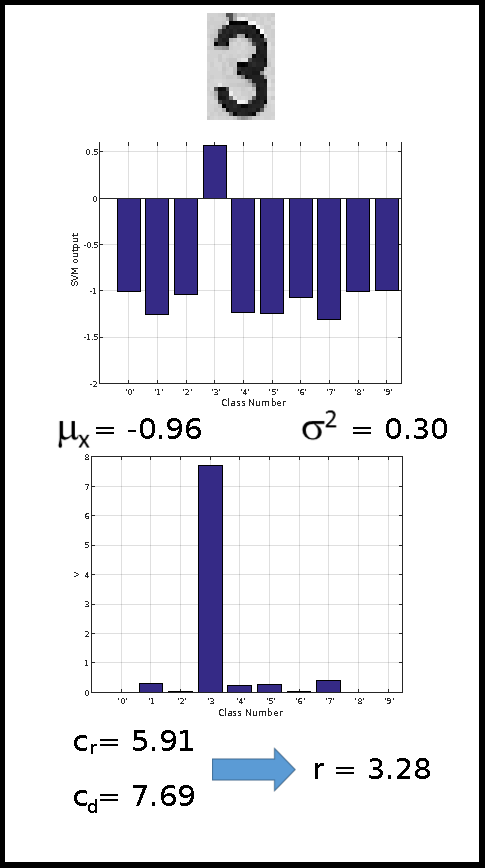
\includegraphics[width=.45\linewidth]{reliability_analysis_3.pdf} & 
			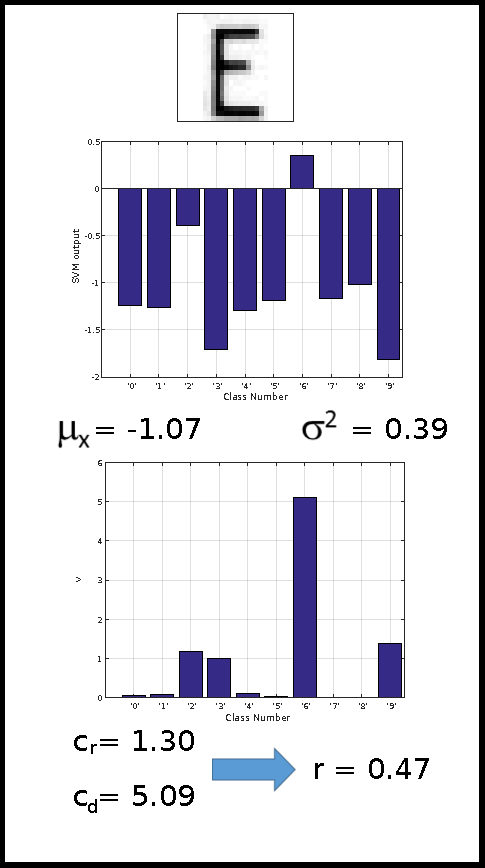
\includegraphics[width=.45\linewidth]{reliability_analysis_E.pdf} \\
		\end{tabular}
\caption{The figure shows two examples of the computation of the reliability measure.}
\label{fig:reliabilityExamples}
\end{center}
\end{figure}


Reliability measure $r<1.0$ could then correspond to a number with a style that is not present in the learning dataset, a wrongly defined bounding box, or an image that is not matched to a number, which is the present case.
If $r>1.0$ the output corresponds to a character with a high discrimination ratio, and can be trusted as a real number.



%------------------------------------------------------------------------------
\section{Experiments and Results}

\subsection{License Plate Number Datasets}

The multi-style license plate dataset is composed of character numbers extracted from the Dlavnekov dataset (USA) \cite{Dlagnekov:dataset,Dlagnekov:2005}, \textit{COMVIS\_cardataset\_v1} (Pakistan) \cite{comvis_dataset}, Medialab's dataset (Greece/Europe) \cite{medialab_greece}, and an Argentinean license plate dataset. 
As can be seen on Fig \ref{fig:dataset}, the license plate numbers of those datasets have opposite colors for the characters and the background.

\begin{figure}[!htbp]
\begin{center}
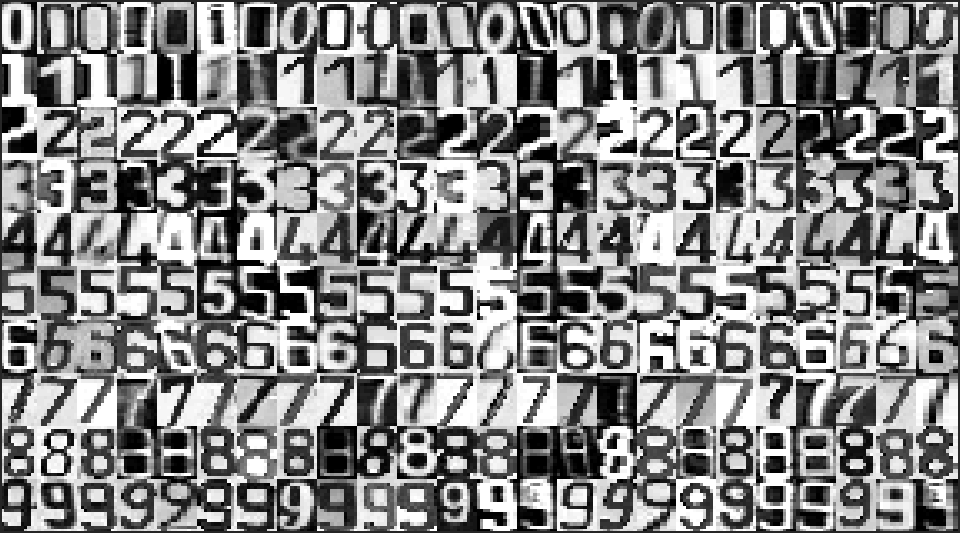
\includegraphics[width=.7\linewidth]{dataset.pdf}
\caption{The figure shows some training and testing samples from the Multi-Style License Plate Numbers dataset, used in the recognition system.}
\label{fig:dataset}
\end{center}
\end{figure}

Table \ref{tab:dataset} details the number of samples for each number class, discriminating between the American, Argentinean, Greek, and Pakistani datasets.

\begin{table}[!htbp]
\small
\begin{center}
\begin{tabular}{l c c c c | l}
\hline
Number & Argentine & USA & Greece & Pakistan & Total\\
\hline
'0' & 33 & 14 & 49 & 19 & 115 \\
'1' & 33 & 22 &  29 & 15 & 99\\
'2' & 42 & 21 & 85 & 30 & 178\\
'3' & 32 & 36 & 74 & 37 & 179\\
'4' & 36 & 61 &  69 & 37 & 203\\
'5' & 32 & 47 &  95 & 21 & 195\\
'6' & 26 & 25 & 75 & 20 & 146\\
'7' & 26 & 25 & 74 & 17 & 142\\
'8' & 30 & 22 & 62 & 35 & 149\\
'9' & 28 & 23 & 74 & 14 & 139\\
\hline
Total & 335 & 310 & 686 & 245 & 1545\\
\hline
\end{tabular}
\caption{This table shows the composition of the License Plate Number Dataset.}
\label{tab:dataset}
\end{center}
\end{table}

%%%%%%%%%%%%%%%%%%%%%%%%%%%%%%%%%%%%%%%%%%%%%%%%%%%%%%%%%%%%%%%%%%%
\subsection{Evaluation of Parameters} \label{sec:evalparams}

This section evaluates the performance of the multiclass SVM classifiers, applying three different kernel functions, increasing the size of the training dataset, and for different values of constant $C$ on the SMO algorithm.

The overall performance of each multi-class classifier is obtained by constructing a confusion matrix of the ten classes.
The Equal Error Rate (EER) is computed as the average of the percentage of samples correctly classified, which are placed at the diagonal of the confusion matrix.

The training is carried out by randomly picking $20$ or $40$ samples per class.
The total number of training samples is then $N=200$ or $N=400$.
The test dataset is built using $50$ remaining samples of each class, and resulting on a total set of $500$ samples.
This operation is repeated three times using different sets of samples.
The performance of each choice is then computed as the mean value of the three EERs.

Linear, Polynomial and Radial Basis Function (RBF) kernels are used below to implement the SVM multi-classification.

\subsubsection*{Linear Kernel Function}

The Linear Kernel function is the simplest similarity measure and is defined by the following equation:
\begin{equation}\label{eq:linkernel}
\K(\x_i,\x_j) = \x_i' \cdot \x_j
\end{equation}

\begin{figure}[!htbp]
	\begin{center}
			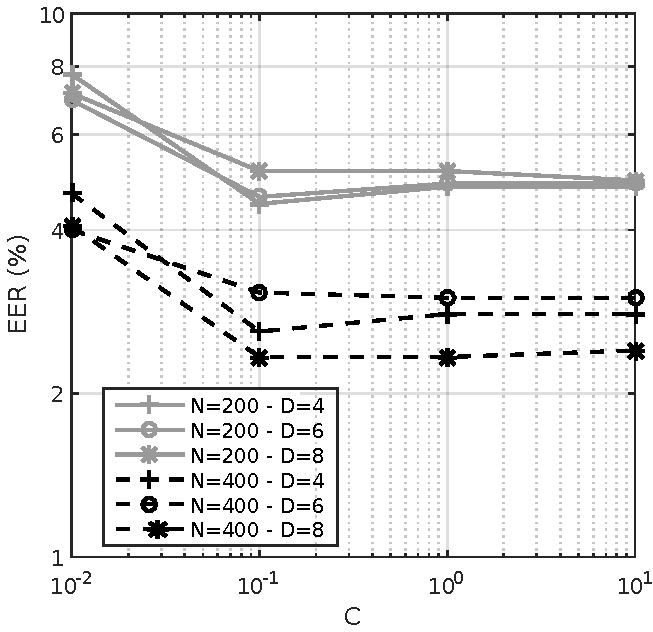
\includegraphics[width=.45\linewidth]{linear_results.pdf}
		\caption{The figure shows the EER of the multi-class license plate number performance using a linear kernel function.}
				\label{fig:linearRes}
	\end{center}
\end{figure}

Fig. \ref{fig:linearRes} shows the performance of the framework using a linear kernel function and changing the number of HOG directions $D$, the $C$ parameter, and the number of training samples ($N$).
The lowest EER value is equal to 2.3 \%.
It is obtained using the largest training dataset with $N=400$, and the more detailed description of the shape with $D=8$.

\subsubsection*{Polynomial Kernel Function}

The Polynomial Kernel function is calculated as:
\begin{equation}
\K(\x_i,\x_j) = (c + \x_i' \cdot \x_j)^d
\end{equation}

\noindent where $d$ is the degree of the polynomial, and $c$ a constant bias which was fixed to $1$ for the tests.

Several tests were conducted using this kernel function and changing parameter $d$ in the polynomial computation, HOG directions values $D$, training dataset size $N$, and SVM constant $C$.
The reliability of the results strongly depend on the degree $d$ of the polynomial function, as can be seen on table \ref{tab:polRelMeasure}.
With $d=2$ (quadratic kernel), the classifiers generalize much better than greater values, obtaining reliable outputs from the SVM classifier.

\begin{table}[!htbp]
\small
	\begin{center}
		\begin{tabular}{c|c}
		{polynomial degree} & Reliable outputs (\%) \\
		\hline
		$d=2$ & 97.6 \\
		$d=3$ & 80.2 \\
		$d=4$ & 74.7 \\
		\hline
		\end{tabular}
		\caption{The table shows the percentage of test samples with valid reliability measure $r>1$.}
				\label{tab:polRelMeasure}
	\end{center}
\end{table}

Fig. \ref{fig:polRes} shows the performance of the classifiers fixing $d=2$ for different values of $C$, $N$ and $D$.
The EER values decrease to $C=10^{-1}$ and stabilize for greater values.
For the smaller dataset ($N=200$), the best accuracy is obtained with $D=4$ HOG directions, with $EER=3.8\%$.
On the other hand, the lowest EER is $2.2\%$ for the larger dataset ($N=400$) and $D=8$ HOG directions. 

\begin{figure}[!htbp]
	\begin{center}
			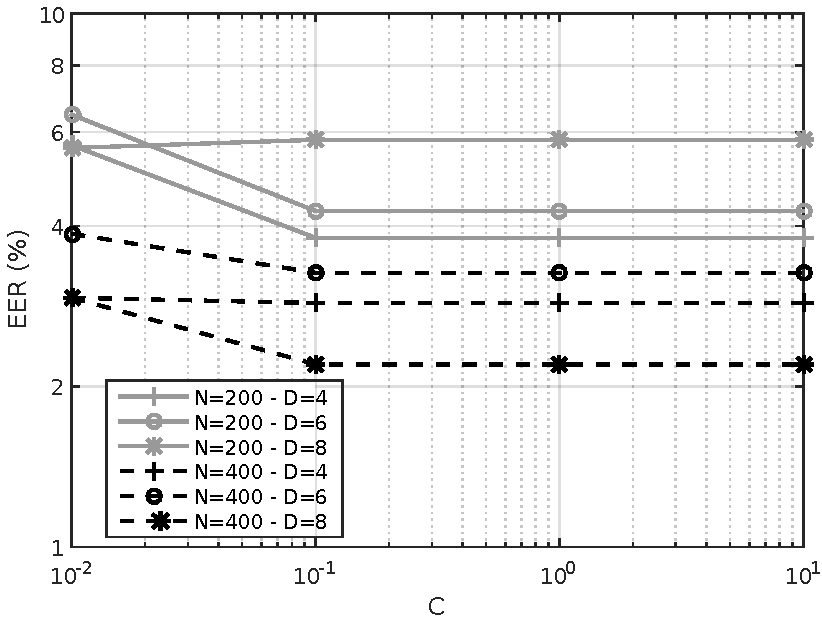
\includegraphics[width=.45\linewidth]{polynomial_results.pdf}
		\caption{The figure presents the EER of the multi-class license plate number performance using polynomial kernel function, with $d=2$.}
				\label{fig:polRes}
	\end{center}
\end{figure}


\subsubsection*{Radial Basis Function Kernel}

The Radial Basis Function (RBF) is widely used in numerous applications with excellent results.
It is considered that this kernel function projects the input feature vector to classification space with infinite dimensions.
The RBF is defined as:
\begin{equation}
\K(\x_i,\x_j) = e^{-\gamma ||\x_i - \x_j||^2}
\end{equation}
\noindent where $\gamma$ is a positive real number.
In general, SVM classifiers using a RBF kernel produce reliable outputs using $r$ measure from equation \ref{eq:reliability}, as can be seen on table \ref{tab:rbfRelMeasure}.
The greatest reliability values are obtained for $\gamma=0.01$.

\begin{table}[!htbp]
\small
	\begin{center}
 		\begin{tabular}{|lcccc}
		\hline
		\backslashbox{$N$}{$\gamma$}						&\multicolumn{1}{|c|}{0.0001} & \multicolumn{1}{|c|}{0.001}  & \multicolumn{1}{|c|}{0.01} & \multicolumn{1}{|c|}{0.1} \\
								\hline
		200 & \multicolumn{1}{|c|}{94.5}&\multicolumn{1}{|c|}{95.4} & \multicolumn{1}{|c|}{99.9} & \multicolumn{1}{|c|}{69.4} \\
		\hline
		400 & \multicolumn{1}{|c|}{98.1}&\multicolumn{1}{|c|}{98.6} & \multicolumn{1}{|c|}{100.0} & \multicolumn{1}{|c|}{82.2} \\
		\hline
		\end{tabular}
		\caption{The table shows the percentage of reliable SVM outputs for an RBF kernel and different parameter values using a reliability measure.}
				\label{tab:rbfRelMeasure}
	\end{center}
\end{table}


Fig. \ref{fig:rbfRes} compares the EER performance for different values on parameters $C$, $N$ and $D$.
The lowest $EER=0.8\%$ is obtained for the larger dataset ($N=400$), for values ($\gamma=0.01$,$D=4$,$C=10$), and set ($\gamma=0.001$,$D=8$,$C=10$).
Using fewer training samples ($N=200$), the performance is similar, obtaining a value of $EER=1.0\%$ for ($\gamma=0.001$,$D=4$,$C=10$) and ($\gamma=0.01$,$D=4$,$C=1$).


\begin{figure}[!htbp]
	\begin{center}
		\begin{tabular}{cc}
			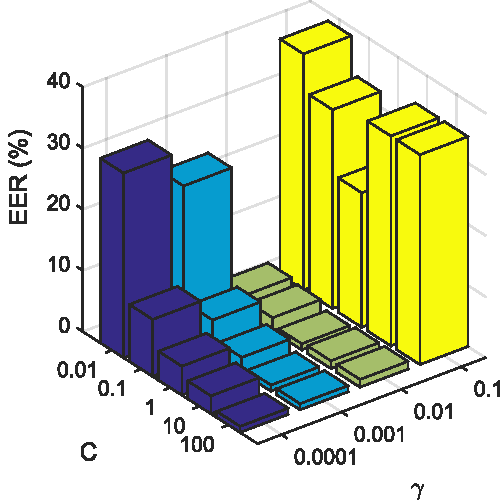
\includegraphics[width=.35\linewidth]{rbf_n200_d4.pdf} &
			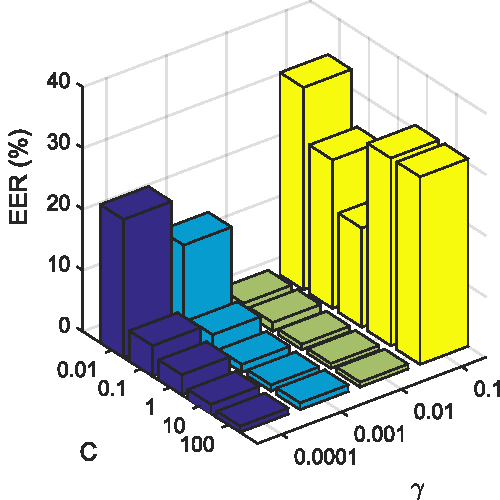
\includegraphics[width=.35\linewidth]{rbf_n400_d4.pdf} \\
			(a) N=200 - D=4 & (b) N=400 - D=4 \\
			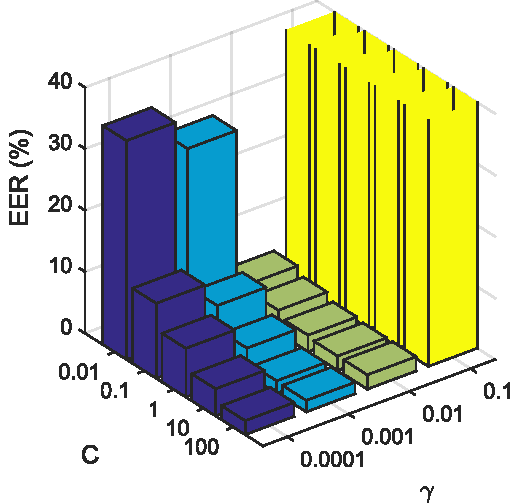
\includegraphics[width=.35\linewidth]{rbf_n200_d8.pdf} &
			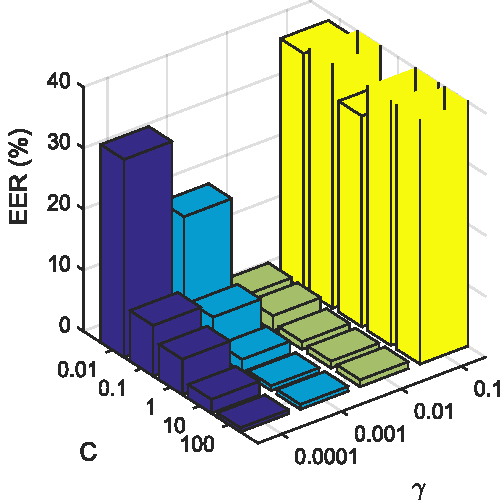
\includegraphics[width=.35\linewidth]{rbf_n400_d8.pdf} \\
			(c) N=200 - D=8 & (d) N=400 - D=8 \\
		\end{tabular}
		\caption{The figure compares the sensibility of the RBF kernel to parameter $C$ for different datasets and input features.}
				\label{fig:rbfRes}
	\end{center}
\end{figure}


\subsection{Operational Complexity and Time Considerations}

Both the operational complexity and processing time depend on the different parameters.
Table \ref{tab:kernelsTime} presents the average processing time, in seconds, to evaluate an input test number in the multi-class recognition number system defined which is composed of different kernel functions and $N$ and $D$ parameters.
The code is entirely written in MATLAB and corresponds to the same that supports this article on IPOL page.
The scripts were executed on an Intel(R) Core(TM) i5 CPU 2.67 GHz, with 4 Gbytes of RAM.

\begin{table}[!htbp]
\small
	\begin{center}
 		\begin{tabular}{|c|c|c|c|}
			      \multicolumn{4}{c}{Linear Kernel} \\
						\hline
		\backslashbox{$N$}{$D$} & 4 & 6 & 8 \\
\hline
$200$ & 0.090 & 0.099 & 0.116 \\
 $400$ & 0.173 & 0.200 & 0.226 \\
\hline
\multicolumn{4}{c}{}\\
			      \multicolumn{4}{c}{Optimized Linear Kernel} \\
						\hline
		\backslashbox{$N$}{$D$} & 4 & 6 & 8 \\
\hline
$200$ & $3.3 \dot 10^{-4}$ & $4.3 \dot 10^{-4}$ & $5.5 \dot 10^{-4}$ \\
 $400$ & $3.7 \dot 10^{-4}$ & $4.5 \dot 10^{-4}$ & $6.2 \dot 10^{-4}$ \\
\hline
\multicolumn{4}{c}{}\\
			      \multicolumn{4}{c}{Polynomial Kernel ($d=2$)} \\
						\hline
		\backslashbox{$N$}{$D$} & 4 & 6 & 8 \\
		\hline
$200$ & 0.109 & 0.122 & 0.136 \\
 $400$ & 0.221 & 0.246 & 0.269 \\
\hline
\multicolumn{4}{c}{}\\
			      \multicolumn{4}{c}{RBF Kernel} \\
						\hline
		\backslashbox{$N$}{$D$} & 4 & 6 & 8 \\
		\hline
$200$ & 0.130 & 0.152 & 0.170 \\
 $400$ & 0.257 & 0.308 & 0.331 \\
\hline
\end{tabular}
\end{center}
\caption{The table shows the average processing time in seconds that it takes to classify a testing sample in the multi-class recognition framework.}
\label{tab:kernelsTime}
\end{table}


The computational complexity of the linear kernel can be estimated by the number of directions $D$, the number of training samples $N$, the number of HOG features $G=871$, and the number of classes $10$.
One linear kernel function call performs $D \times G$ sums and $D \times G$ products.
The SVM output, as shown in eq. \ref{eq:svmoutput}, adds $2 \times N$ products, corresponding to labels $y_i$ and alphas $\alpha_i$, and $N$ sums.
Thus, it takes $N \times D \times G+N$ sums, and $N \times D \times G+2 \times N$ multiplications to obtain an individual output.
To classify one testing sample, the framework will perform this operation $10$ times.
The complexity has an order of $10 \times N \times D \times G$ sums and $10 \times N \times D \times G$ multiplications.

There are some options to reduce the computational complexity. 
Firstly, eq. \ref{eq:svmoutput} can be solved by only using support vectors: those training samples with $\alpha_i \neq 0$.
Depending on the problem, this can consist of a 10 \% reduction in the number of operations.
Secondly, Platt proposes an optimization for linear kernels.
Using eq. \ref{eq:linkernel}, evaluation function \ref{eq:svmoutput} becomes:
\begin{equation}\label{eq:linsvmoutput}
f(\x_t)= sign \left(\sum_{i=1}^N y_i \alpha_i \\ \x_t \cdot \x_i - b\right)
\end{equation}
Eq. \ref{eq:linsvmoutput} is linear and can be solved using a single weight vector $\w$:
\begin{equation}\label{eq:fastlinsvmoutput}
f(\x_t)= sign \left(\w \cdot \x_t - b\right)
\end{equation}

This drastically reduces the number of operations to $10 \times D \times G$ sums and $10 \times D \times G$ products.

The processing time to evaluate one example using an RBF kernel is by far the longest, considering the linear kernel optimization.
The use of this kernel function represents a compromise between good performance and fast response.
If the application does not need real time outputs, the RBF kernel represents a very good choice.

\subsection{Results}

This section presents the results obtained by running the Multi-Style License Number Recognition Framework IPOL code supporting this article.


\begin{table}[!h]
  \begin{center}
	\begin{tabular}{| l| l | c|}
    	\hline
			Feature & Classification Method & Accuracy (\%) \\
    	\hline
 Raw data & Knn (K=5)  &         79.1 \\
HOG & Knn (K=5)   &         96.8 \\
Raw data & SVM  &         91.7 \\
HOG & SVM  & \textbf{99.0} \\
    	\hline
	\end{tabular}
  \end{center}
  \caption{Comparing classification results using HOG features and intensity raw values, and SVM against KNN classifiers.}
  \label{tab:CompRes}
\end{table}


Table \ref{tab:CompRes} compares HOG features results against intensity raw values using two classification methods.
Because the images of the character numbers have different sizes, they were resized to $16 \times 12$ pixels, to get an intensity feature vector with the same length.
SVM is compared with a simple K-Nearest Neighbors (KNN) classification using $K=5$.
For HOG features, histogram distances are calculated using vector correlation, and for intensity features, the euclidean distance of the normalized pixels values.
The overall performance of each system is evaluated by computing the classification rate of each number, then the mean of the diagonal of the confusion matrix.
Table \ref{tab:MatConf} shows the results on the corresponding confusion matrix using SVM classifier and HOG features, which yields the highest accuracy ratio.

The default kernel function for the SVM classifier is the RBF, with $\gamma = 0.01$, constant $C=1$, and the number of HOG directions is $D=4$.
The training dataset is composed of $N=200$ randomly chosen samples, consisting of $20$ elements per class number.
The remaining samples will make up the test set.


Results are very good, even if the number of training samples is very limited.
This can be explained because LPR numbers should have standard shapes following the country regulations.
It simplifies the generalization of the classes shape using HOG features, compared with intensity values.
Finally, it is not then necessary to have a large training set, as the shapes of the same numbers have very similar features.

\begin{table}[!h]
  \begin{center}
	\begin{tabular}{| l| c| c| c| c| c| c|c|c| c|c|}
    	\hline
    	         & '0' & '1' & '2' & '3' & '4' & '5' & '6' & '7' & '8' & '9'\\
    	  \hline
			'0'     & \textbf{100.0}  &   0.0  &   0.0  &   0.0  &   0.0  &   0.0  &   0.0  &   0.0  &   0.0  &   0.0   \\
			'1'   & 0.0  &  \textbf{97.3}  &   0.0  &   0.0  &   2.7  &   0.0  &   0.0  &   0.0  &   0.0   &  0.0   \\
			'2'     & 0.0  &   0.0 &  \textbf{99.4}  &   0.0  &   0.0  &   0.0  &   0.0  &   0.6  &   0.0  &   0.0   \\
			'3'       & 0.0  &   0.0  &   0.0 &  \textbf{98.7}  &   0.0  &   0.7  &   0.0  &   0.7  &   0.0  &   0.0 \\
			'4'      & 1.1   &  0.0  &   0.6  &   0.0 &  \textbf{98.3}  &   0.0  &   0.6  &   0.0  &   0.0  &   0.0    \\
			'5'    & 0.0  &   0.0  &   0.0  &   0.0  &   0.0  & \textbf{100.0}  &   0.0  &   0.0  &   0.0   &  0.0     \\
			'6'    & 0.0  &   0.0  &   0.0  &   0.0  &   0.0  &   0.9  & \textbf{99.1}  &   0.0  &   0.0  &   0.0   \\
			'7'       & 0.0   &  0.0  &   0.0  &   0.0  &   0.0   &  0.0  &   0.0  & \textbf{100.0}  &   0.0  &   0.0 \\
			'8'      & 0.0  &   0.0  &   0.0  &   0.0  &   0.0  &   0.0  &   0.8  &   0.0 &  \textbf{99.2}  &   0.0   \\
			'9'    & 0.0  &   0.0  &   0.9  &   0.0  &   0.0  &   0.0  &   0.0  &   0.0  &   0.9 &  \textbf{98.1}     \\
       \hline 
	\end{tabular}
  \end{center}
  \caption{Confusion matrix of License Plate Number recognition in the test samples from the four datasets.}
  \label{tab:MatConf}
\end{table}

The reliability measure, using eq. \ref{eq:reliability} for the SVM classifier using HOG features, is computed in each test sample.
The percentage of samples with $r>1.0$ is 93 \%.



%------------------------------------------------------------------------------
\section*{Image Credits}
The multi-style license plate dataset \textit{COMVIS\_cardataset\_v1} and the Medialab's dataset are provided without license.
The Argentinean dataset is also distributed without license.
Dlavnekov's dataset can be freely employed for research purposes.

%------------------------------------------------------------------------------
\bibliographystyle{siam}
\bibliography{article}

\end{document}
%------------------------------------------------------------------------------
